\documentclass[10pt,border=4pt]{standalone}
\usepackage{mathptmx}
\usepackage{amsmath,amssymb,bm}
\usepackage{tikz}
\usetikzlibrary{patterns,decorations.pathmorphing,decorations.pathreplacing,arrows.meta,fit,backgrounds,calc,positioning,shapes.geometric}
\definecolor{acc}{HTML}{0B5394}
\definecolor{accl}{HTML}{EAF0F7}
\definecolor{grp}{HTML}{F5F5F5}
\definecolor{org}{HTML}{C55A11}
\definecolor{orgl}{HTML}{FBEFE6}
\tikzset{
 dat/.style={draw=black,line width=0.6pt,fill=white,align=center,font=\small,inner sep=3pt,minimum height=0.85cm},
 lay/.style={draw=acc,line width=0.8pt,fill=accl,rounded corners=2pt,align=center,font=\small,inner sep=3pt,minimum height=0.85cm},
 cnd/.style={draw=org,line width=0.8pt,fill=orgl,rounded corners=2pt,align=center,font=\small,inner sep=3pt,minimum height=0.75cm},
 op/.style={circle,draw=black,line width=0.6pt,fill=white,inner sep=0.5pt,font=\small,minimum size=5mm},
 grpb/.style={draw=black!45,dashed,line width=0.6pt,rounded corners=3pt,inner sep=6pt},
 arr/.style={-{Latex[length=2.2mm,width=1.7mm]},line width=0.7pt},
 carr/.style={-{Latex[length=2.2mm,width=1.7mm]},line width=0.7pt,draw=org},
 shp/.style={font=\scriptsize,text=black!70,inner sep=1pt},
 lab/.style={font=\footnotesize,inner sep=1pt},
 ttl/.style={font=\small\bfseries,inner sep=0pt,anchor=west}
}
\newcommand{\xh}{\mathbf{x}_h}\newcommand{\xf}{\mathbf{x}_f}

\begin{document}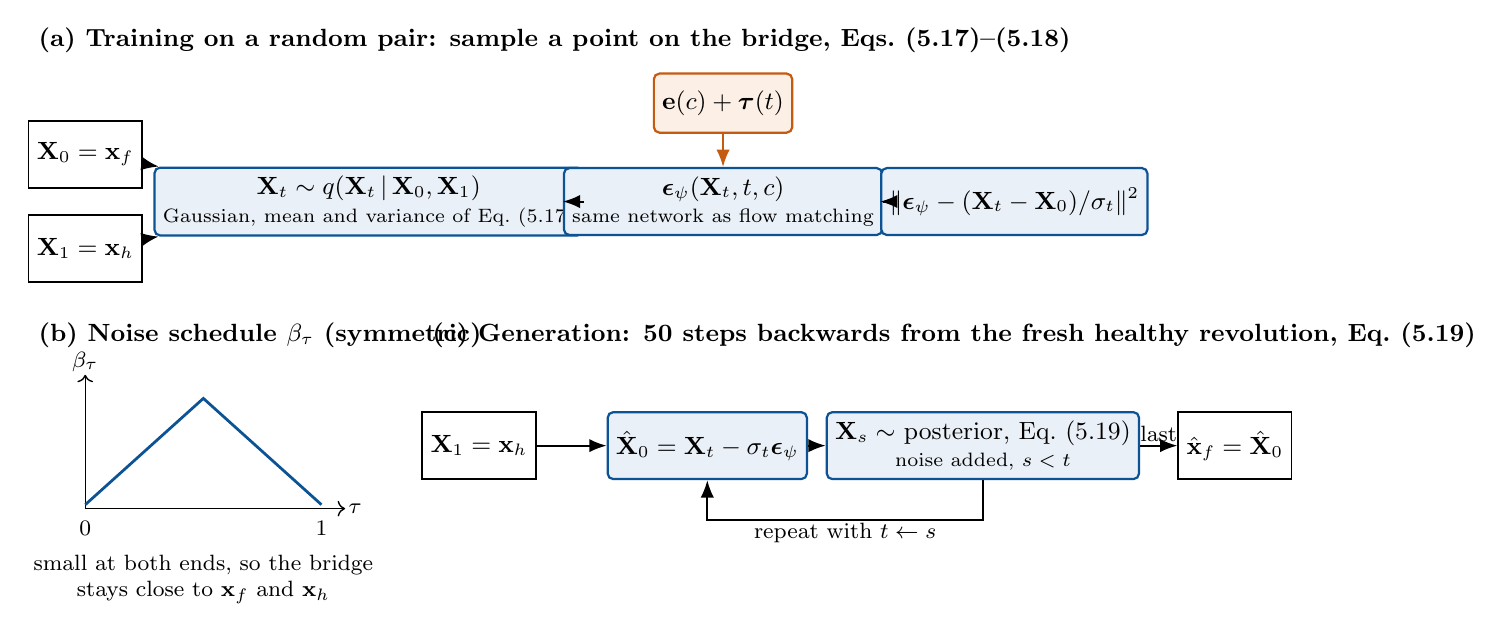
\begin{tikzpicture}[x=1cm,y=1cm]
\node[ttl] at (-0.6,1.75) {(a) Training on a random pair: sample a point on the bridge, Eqs.~(5.17)--(5.18)};
\node[dat] (x0) at (0,0.3) {$\mathbf{X}_0=\xf$};
\node[dat] (x1) at (0,-0.9) {$\mathbf{X}_1=\xh$};
\node[lay] (br) at (3.6,-0.3) {$\mathbf{X}_t\sim q(\mathbf{X}_t\,|\,\mathbf{X}_0,\mathbf{X}_1)$\\[-1pt]\scriptsize Gaussian, mean and variance of Eq.~(5.17)};
\node[lay] (net) at (8.1,-0.3) {$\boldsymbol\epsilon_\psi(\mathbf{X}_t,t,c)$\\[-1pt]\scriptsize same network as flow matching};
\node[lay] (loss) at (11.8,-0.3) {$\lVert\boldsymbol\epsilon_\psi-(\mathbf{X}_t-\mathbf{X}_0)/\sigma_t\rVert^2$};
\draw[arr] (x0)--(br); \draw[arr] (x1)--(br); \draw[arr] (br)--(net); \draw[arr] (net)--(loss);
\node[cnd] (c) at (8.1,0.95) {$\mathbf{e}(c)+\boldsymbol\tau(t)$}; \draw[carr] (c)--(net);
% schedule sketch
\node[ttl] at (-0.6,-2.0) {(b) Noise schedule $\beta_\tau$ (symmetric)};
\draw[->,line width=0.5pt] (0,-4.2)--(3.3,-4.2) node[lab,right]{$\tau$}; \draw[->,line width=0.5pt] (0,-4.2)--(0,-2.5) node[lab,above]{$\beta_\tau$};
\draw[line width=1pt,acc] (0,-4.15)--(1.5,-2.8)--(3.0,-4.15);
\node[lab] at (0,-4.45) {0}; \node[lab] at (3.0,-4.45) {1}; \node[lab,align=center] at (1.5,-5.1) {small at both ends, so the bridge\\stays close to $\xf$ and $\xh$};
% generation
\node[ttl] at (4.4,-2.0) {(c) Generation: 50 steps backwards from the fresh healthy revolution, Eq.~(5.19)};
\node[dat] (s) at (5.0,-3.4) {$\mathbf{X}_1=\xh$};
\node[lay] (p1) at (7.9,-3.4) {$\hat{\mathbf{X}}_0=\mathbf{X}_t-\sigma_t\boldsymbol\epsilon_\psi$};
\node[lay] (p2) at (11.4,-3.4) {$\mathbf{X}_s\sim$ posterior, Eq.~(5.19)\\[-1pt]\scriptsize noise added, $s<t$};
\node[dat] (o) at (14.6,-3.4) {$\hat{\mathbf{x}}_f=\hat{\mathbf{X}}_0$};
\draw[arr] (s)--(p1); \draw[arr] (p1)--(p2); \draw[arr] (p2)--node[lab,above]{last}(o);
\draw[arr] (p2.south) -- ++(0,-0.5) -| node[lab,below,pos=0.25]{repeat with $t\leftarrow s$} (p1.south);
\end{tikzpicture}\end{document}
